\section{Introduction}
In a cluster-based cloud environment,
% such as ones provided by Amazon EC2\cite{AmazonEC2} and Alibaba Aliyun\cite{Aliyun},
each physical machine runs a number  of virtual machines as  instances of a guest operating system 
and their  virtual hard disks are represented as virtual disk image files in the host operating system.
%virtual disk image files (e.g. .vhd, .vmdk) in the host operating system.
%Backup  of virtual disks is relatively straightforward since
%these image files are stored as regular files from the external point of view,
%backing up VM's data is mainly done by taking snapshots of virtual disk images.
%A snapshot preserves the data of a VM's file system at a specific point in time. 
%VM snapshots can be  backed up  incrementally by comparing blocks from one version to another 
%and only the blocks that have changed from the previous version of snapshot will be saved~\cite{Clements2009,Vrable2009}. 
Frequent  snapshot backup of virtual disk images  can increase  the service reliability. 
For example, the Aliyun cloud, which is  the largest cloud service provider by Alibaba in China, 
automatically conducts  the backup of virtual disk images to all active users every day.
The cost of supporting a large number of concurrent backup streams is high
because of the huge storage demand. 
Using a separate  backup service with full deduplication support~\cite{venti02,bottleneck08}
%(Figure~\ref{fig:traditional-arch})
can effectively identify and remove content duplicates among snapshots, 
but such a solution can be expensive. There is also a large amount of 
network traffic to transfer  data from the host machines to the backup facility
before duplicates are removed.

%\begin{figure}[htb]
%    \centering
%    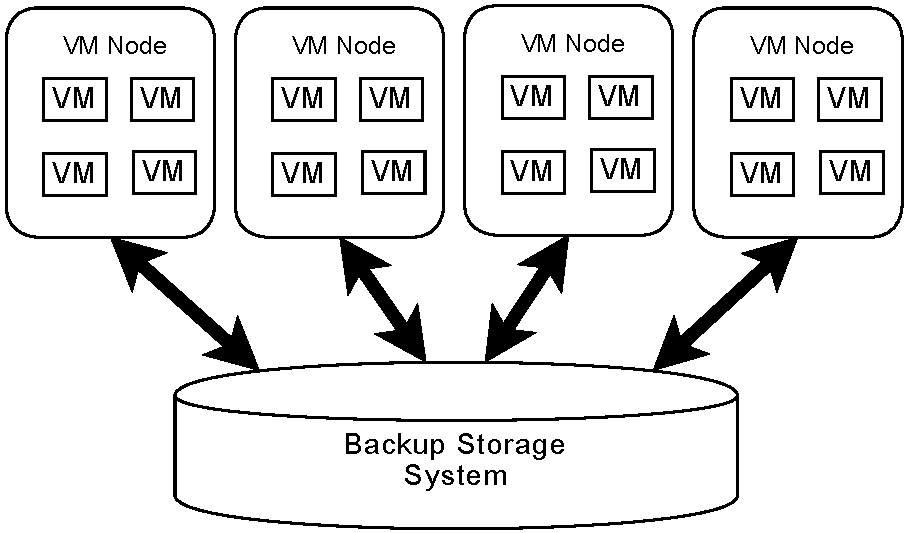
\includegraphics[width=3in]{images/traditional-arch}
%    \label{fig:traditional-arch}
%    \caption{Traditional VM Backup System}
%\end{figure}


This paper seeks for a low-cost architecture option  that collocates
a backup service with other cloud services and  uses a minimum amount of resources. 
%Since most of backup data is not used in practice, system resource in such a service is not fully utilized.
%The dirty bit approach~\cite{??}  which checks the version difference can effectively remove
%duplicates while using content fingerprints can significantly compress more~\cite{Bottlneck08}.
%On the other hand, comparing fingerprints  adds significant  memory cost. 
%Since each physical machine in a cluster  hosts many VMs, memory contention happens frequently.
%Cloud providers often wish that the backup service only consumes  small or modest resources
%with a minimal impact to the existing cloud services.  
%We study and evaluate the integration of several deduplication strategies to meet
%the low-cost collocation requirement. 
%A recent study using subsampling~\cite{Guo2011}  can significantly reduce the memory requirement.
We also consider the fact that after
deduplication, most data chunks are shared by several to many virtual machines.
Failure of few shared data chunks can have a 
%catastrophic 
broad effect and many
snapshots of virtual machines would be affected.
The previous work in deduplication focuses on the efficiency and approximation of
finger print comparison, and has not addressed fault handling issues  together with deduplication.
Thus we also seek deduplication options that yield better fault isolation.
% along with a low-cost solution.
Another issue considered is that
that deletion of old snapshots compete for computing resource as well. 
%That is because data dependence created deletion of old snapshots competes for computing resources.
% as well so deletion needs to be considered in system design. 
Sharing of data chunks among by multiple VMs needs to be detected during
snapshot   deletion and such dependence complicates deletion operations. 
%The additional complexity for deletions
%come from the dependencies created by multiple links to the same problem, so
%some solution is needed to determine blocks with no dependent snapshots after deletion.
%especially when  VMs can migrate around in the cloud.

%\begin{figure}[htb]
%    \centering
%    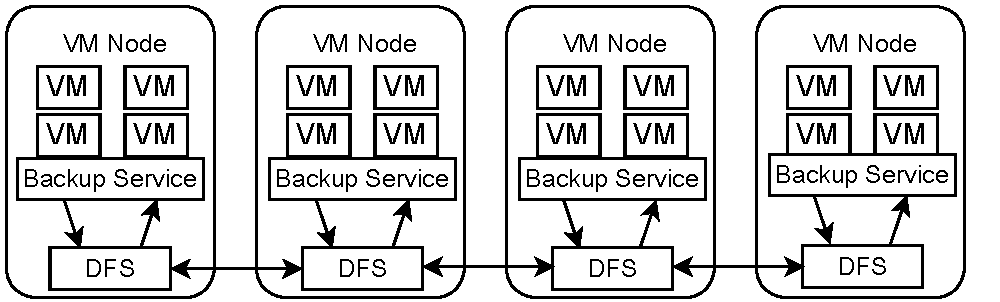
\includegraphics[width=3in]{images/colocated-arch}
%    \label{fig:colocated-arch}
%    \caption{Collocated VM Backup System}
%\end{figure}

The paper studies and evaluates  an integrated approach which uses  multiple duplicate detection strategies
based on  version  detection, inner VM duplicate search,
and controlled cross-VM comparison. 
This approach is VM centric by localizing duplicate detection within each VM  
and by packaging data chunks from the same VM into a file system block as much as possible.
By narrowing duplicate sharing within a small percent of common data chunks and exploiting their popularity,
this scheme can afford to allocate extra replicas of these shared chunks for better
fault resilience while sustaining competitive deduplication efficiency.
Localization also brings the benefits of greater ability to exploit parallelism so
backup operations can run simultaneously without a central  bottleneck.
This  VM-centric solution uses  a small amount of  memory while delivering a reasonable deduplication efficiency. 
%Our deletion strategy uses a double Bloom filter strategy for periodic mark-and-sweeping of expired data.
We have developed a prototype system that runs a cluster of Linux machines with Xen and uses 
a standard distributed file system for the backup storage. 
% with data replication and block packaging.
%and we allocate more  replicas for the commonly-shared  data 
%blocks among VM snapshots to enhance fault tolerance.



%************** Paper sections summary
%THIS NEEDS MODIFICATION
The rest of this paper is organized as follows.
Section~\ref{option} reviews the background and discusses the  design options for snapshot backup 
with a VM-centric approach. 
Section~\ref{sect:model}  analyzes the tradeoff and benefit of our approach. 
Section~\ref{sect:arch}  describes our system architecture and implementation details.
%   the benefit of our approach for fault isolation. 
Section~\ref{exper} is our experimental evaluation that compare with the other approaches.
Section~\ref{conc}  concludes this paper.

%We are seeking Unlike the previous work dealing with general file-level backup and deduplication, our problem is focused on 
%virtual disk image backup. Although we treat each virtual disk  as a file logically, its size is very large.
%On the other hand, we need to support parallel backup of a large number of virtual disks in a cloud every day. 
%One key requirement we face at Alibaba Aliyun is that VM snapshot backup should only use a minimal amount of system
%resources so that most of resources is kept for regular cloud system services or applications.
%Thus our objective is to exploit the characteristics of VM snapshot data and
%pursue a cost-effective deduplication solution. 
%Another goal  is to decentralize VM snapshot backup and  localize  deduplication as much as possible,

%,extreme_binning09,sparseindex09
\comments{
By observations on the VM snapshot data from production cloud, we found snapshot data duplication 
can be easily classified into two categories: \emph{inner-VM} and \emph{cross-VM}. Inner-VM duplication
exists between VM's snapshots, because the majority of data are unchanged during each backup period. 
On the other hand, Cross-VM duplication is mainly due to widely-used software and libraries such as Linux and MySQL.
As the result, different VMs tend to backup large amount of highly similar data.

With these in mind, we  have developed a distributed multi-level solution to conduct 
segment-level  and block-level inner-VM  deduplication to localize the deduplication effort when possible.
It then makes cross-VM deduplication by excluding a small number of
popular common data blocks from being backed up. Our study shows that common data blocks
occupy significant amount of storage space while they only take
a small amount of resources to deduplicate.
Separating deduplication into multi levels effectively accomplish the major space saving goal
compare the global complete deduplication scheme, at the same time it makes
the backup of different VMs to be independent for better fault tolerance.

The following table shows the strength and weakness of some well-know deduplication systems:
\begin{table}
    \begin{tabular}{|l|l|l|l|}
        \hline
        ~           & Scalability & Low-cost & Full Dedup \\ \hline
        DDFS        & N           & N        & Y          \\ 
        Ex-bin      & Y           & Y        & N          \\ 
        Guo         & Y           & N        & N          \\ 
        iDedup      & N           & Y        & N          \\ 
        Founadation & N           & N        & Y          \\
        \hline
    \end{tabular}
\end{table}
}
